\subsection{下降：覆叠的情形}

设 X、Y 是拓扑空间，且 \(f: X \to Y\) 是满射连续映射。设 \((Z, p)\) 是 X 的覆叠，\(\tau\) 是关于 f 在 Z 上的下降数据。

若 \(f\) 是逆紧且分离的（相应地，若 \(f\) 是开映射），则下降数据 \(\tau\) 是有效的，且 Y-空间 \(Z/R_{\tau}\) 是平展空间（IV, 第~389~页，命题 5）。如果 \(f\) 在每一点的某个邻域内有连续截面（I, 第~72~页，命题 3），或者 Z 是 X 的局部有限覆叠（I, 第~77~页，推论 4），那么它甚至是 Y 的覆叠。本节旨在说明使 \(Z/R_{\tau}\) 成为 Y 的覆叠的其他条件。

首先证明一个引理。

引理 1. --- 设 B、B' 是拓扑空间，且 \(f: \mathrm{B}' \to \mathrm{B}\) 是连续映射。如果纤维方块 \(\mathrm{B}' \times_{\mathrm{B}} \mathrm{B}'\) 是局部连通的，则拓扑空间 \(\mathrm{B}'\) 是局部连通的。

设 \(a\) 是 \(\mathrm{B}'\) 中的一点，V 是 \(a\) 的一个邻域。假设纤维方块 \(\mathrm{B}' \times_{\mathrm{B}} \mathrm{B}'\) 是局部连通的，并令 W 是 \((a, a)\) 在 \(\mathrm{B}' \times_{\mathrm{B}} \mathrm{B}'\) 中的一个连通邻域，且包含于 \(\mathrm{V} \times \mathrm{V}\) 中。置 \(\mathrm{U} = \mathrm{pr}_1(\mathrm{W})\)。集合 U 包含于 V 中，并且是连通的，因为连通集在连续映射下的像是连通的。若 \(\Delta_{\mathrm{B}'}\) 表示 \(\mathrm{B}' \times_{\mathrm{B}} \mathrm{B}'\) 的对角线，则映射 \(\mathrm{pr}_1 \mid \Delta_{\mathrm{B}'}: \Delta_{\mathrm{B}'} \to \mathrm{B}'\) 是同胚。由于 U 包含 \(\mathrm{pr}_1(\mathrm{W} \cap \Delta_{\mathrm{B}'})\)，且 \(\mathrm{W} \cap \Delta_{\mathrm{B}'}\) 是 \((a, a)\) 在 \(\Delta_{\mathrm{B}'}\) 中的一个邻域，所以 U 是 \(a\) 在 \(\mathrm{B}'\) 中的一个邻域。这就证明了引理。

命题 6. --- 设

\pandocbounded{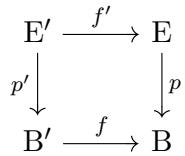
\includegraphics[keepaspectratio]{images/part003_c1a9b5e7.jpg}}

为一个笛卡尔方块。我们假设映射 f 是逆紧、分离且满射的，并作出下列假设之一：

\begin{enumerate}
\def\labelenumi{(\roman{enumi})}
\item
  f 的纤维是局部连通的，且纤维方块 \(B^{\prime} \times_{B} B^{\prime}\) 是局部连通的。
\item
  \(f\) 的纤维是有限的，\(\Delta_{\mathrm{B}^{\prime}}\) 是 \(\mathrm{B}^{\prime}\times_{\mathrm{B}}\mathrm{B}^{\prime}\) 的对角线，且在 \(\mathrm{B}^{\prime}\times_{\mathrm{B}}\mathrm{B}^{\prime}\) 中是开集，并且 \(\mathrm{B}^{\prime}\times_{\mathrm{B}}\mathrm{B}^{\prime} - \Delta_{\mathrm{B}^{\prime}}\) 是局部连通空间。
\end{enumerate}

那么，若 \((\mathrm{E}^{\prime}, p^{\prime})\) 是覆叠，\((\mathrm{E}, p)\) 也是覆叠。

由于映射 \(f\) 是万有严格的（I, 第~20~页，推论），映射 \(p\) 是平展的（I, 第~31~页，命题 8）且分离的（I, 第~27~页，命题 4）。不妨设 \(\mathrm{E}' = \mathrm{B}' \times_{\mathrm{B}} \mathrm{E}\)。

设 \(a\) 是 B 中一点；目标是证明点 \(a\) 有一个邻域 W，使得 W-空间 \((\mathrm{E_W}, p_{\mathrm{W}})\) 是可平凡化的覆叠。令 \(\mathrm{B}_a^\prime = f^{-1}(a)\)，并令 \(\mathrm{E}_a^\prime = (p')^{-1}(\mathrm{E}_a)\)。映射 \(t_a: \mathrm{E}_a^\prime \to \mathrm{B}_a^\prime \times \mathrm{E}_a\) 由 \(t_a(y) = (p'(y), f'(y))\) 定义，是一个 \(\mathrm{B}_a^\prime\)-同构（I, 第~9~页，命题 4），因此 \(\mathrm{E}_a^\prime\) 是 \(\mathrm{B}_a^\prime\) 的可平凡化覆叠，而 \(t_a\) 是此覆叠的平凡化。

证明存在一个邻域 \(V'\)，它是 \(B'_{a}\) 在 \(B'\) 中的邻域，以及覆叠（\(E_{V'}', p_{V'}\)）的一个连续平凡化 t，使其延拓 \(t_{a}\)。在假设（ii）下，\(B'_{a}\) 是有限的，且其中各点有两两不交的开邻域，在这些邻域上覆叠 \(E'\) 可平凡化，故此情形下断言成立。在假设（i）下，\(B'_{a}\) 是局部连通的，B' 也是如此（IV, 第~390~页，引理 1）；由于映射 f 逆紧且分离，\(B'_{a}\) 是紧的，且任意两个不同的点在 B' 中有不交邻域，从而偶对（B', \(B'_{a}\)）满足性质（PCV）（I, 第~37~页，引理 1）。因此断言由 I, 第~90~页推论 2 得出。

由于 \(f\) 逆紧，存在一个邻域 \(V\)，它是 \(a\) 在 \(B\) 中的邻域，使得 \(V'\) 包含 \(f^{-1}(V)\)（I, 第~75~页，引理）。因此不妨设 \(V' = f^{-1}(V)\)。

给 \(V'\)-空间 \(V' \times E_{a}\) 和 \(E_{V'}' = V' \times_{B} E\) 赋予关于 \(f_{V}: V' \to V\) 的规范下降数据。我们要证明，可能缩小 V 和 \(V'\) 后，刚定义的 \(V'\)-空间同构 \(t: E_{V'}' \to V' \times E_{a}\) 与下降数据相容，即有 \(t(b_{1}', x) = t(b_{2}', x)\)，只要 \((b_{1}', b_{2}') \in V' \times_{V} V'\) 且 \(x \in E_{f(b_{1}')}\)。记 \(\widetilde{t}\) 为映射 \(pr_{2} \circ t: E_{V'}' \to E_{a}\)。

令 \(V'' = V' \times_{V} V'\)；通过第一投影将其视为 \(V'\)-空间。映射 \(((b_{1}', b_{2}'), x) \mapsto ((b_{1}', b_{2}'), (b_{1}', x))\)，从 \(V'' \times_{V} E\) 到 \(V'' \times_{V'} E'\)，是 \(V''\)-空间的同构；这说明 \(V'' \times_{V} E\) 是 \(V''\) 的覆叠。

对 \(i=1,2\)，定义映射 \(u_{i}\colon V^{\prime\prime}\times_{V}E\to V^{\prime\prime}\times E_{a}\)，令 \(u_{i}(b_{1}^{\prime},b_{2}^{\prime},x)=(b_{1}^{\prime},b_{2}^{\prime},\widetilde{t}(b_{i}^{\prime},x))\)；它们是覆叠 \(V^{\prime\prime}\times_{V}E\) 的平凡化。令 \(W^{\prime\prime}\) 为点 \(w\in V^{\prime\prime}\) 的集合，在这些点上平凡化 \(u_{1}\) 和 \(u_{2}\) 重合；它包含 \(B_{a}^{\prime}\times B_{a}^{\prime}\)，也包含对角线 \(\Delta_{V'}\)。证明 \(W^{\prime\prime}\) 是 \(B_{a}^{\prime}\times B_{a}^{\prime}\) 的一个邻域。在假设（i）下，这由 I, 第~80~页推论 2 得出，因为 \(B^{\prime}\times B^{\prime}\) 是局部连通的。在假设（ii）下，\(W^{\prime\prime}\) 包含 \((B_{a}^{\prime}\times B_{a}^{\prime})-\Delta_{B_{a}^{\prime}}\) 在 \((B^{\prime}\times_{B}B^{\prime})-\Delta_{B^{\prime}}\) 中的一个邻域，因为这个集合是局部连通的（同上）。由于 \(\Delta_{V'}\) 在 \(B^{\prime}\times_{B}B^{\prime}\) 中开，\(W^{\prime\prime}\) 是 \(B_{a}^{\prime}\times B_{a}^{\prime}\) 在 \(V^{\prime\prime}\) 中的一个邻域。

由于 \(f\) 逆紧，规范映射 \(f''\) 将 \(\mathrm{B}' \times_{\mathrm{B}} \mathrm{B}'\) 映到 B，并且是逆紧的，因为它是投影 \(\mathrm{pr}_{1} \colon \mathrm{B}' \times_{\mathrm{B}} \mathrm{B}' \to \mathrm{B}'\) 与映射 \(f\) 的复合。

根据 I, 第~75~页的引理，存在 V 中 a 的一个邻域 W，使得 \((f'')^{-1}(\mathrm{W})\) 包含于 \(W''\)；令 \(W'=(f')^{-1}(\mathrm{W})\)，它是 \(V'\) 的子集，且平展空间同构 \(t: E_{W'}' \to W' \times E_a\) 与关于映射 \(f_W: W' \to W\) 的规范下降数据相容。根据推论（IV, 第~388~页），

W-平展空间 \(E_{W}\) 和 \(W \times E_{a}\) 同构。特别地，\(E_{W}\) 是可平凡化覆叠，命题得证。

推论 1. --- 设 E 和 B 是拓扑空间，\(p\colon\mathrm{E}\to\mathrm{B}\) 是连续映射，且 \((\mathrm{A}_{i})_{i\in\mathrm{I}}\) 是 B 的局部有限闭覆盖，使得对每一对 \((i,j)\in\mathrm{I}\times\mathrm{I}, i\neq j\)，交集 \(\mathrm{A}_{i}\cap\mathrm{A}_{j}\) 是局部连通空间。那么，B-空间 \((\mathrm{E},p)\) 是覆叠的必要且充分条件是：对每个 \(i\in\mathrm{I}\)，\(\mathrm{A}_{i} \)-空间 \((p^{-1}(\mathrm{A}_{i}),p_{\mathrm{A}_{i}})\) 是 \(\mathrm{A}_{i}\) 的覆叠。

这个条件是必要的（参见 I, 第~69~页）。反之，令 B' 为族 \((\mathrm{A}_{i})_{i\in\mathrm{I}}\) 的拓扑和空间，令 \(f\colon B'\to B\) 为规范映射。映射 f 是闭的（TG, I, 第~6~页，命题 4）、分离的（I, 第~27~页，注 5），具有有限纤维，因而是逆紧的（TG, I, 第~75~页，定理 1）；它还是满射。对角线 \(\Delta_{B'}\) 等于 \(\bigcup_{i\in I}A_{i}\times_{B}A_{i}\)，所以在 \(B'\times_{B}B'\) 中是开集。最后，空间 \((\mathrm{B}'\times_{\mathrm{B}}\mathrm{B}')-\Delta_{\mathrm{B'}}\) 同胚于族 \((\mathrm{A}_{i}\cap\mathrm{A}_{j})\)、\((i,j)\in\mathrm{I}\times\mathrm{I}\)、\(i\neq j\) 的和空间；因而是局部连通的。命题 6 的假设（ii）得到满足。若对每个 i，\(p^{-1}(\mathrm{A}_{i})\) 是 \(A_{i}\) 的覆叠，则 \(E'\) 是 \(B'\) 的覆叠，故 E 是 B 的覆叠。

推论 2. --- 设 X 和 Y 是拓扑空间，设 \(f\colon X \to Y\) 是逆紧、分离且满射的映射。此外，假设下列假设之一成立：

\begin{enumerate}
\def\labelenumi{(\roman{enumi})}
\item
  f 的纤维以及空间 \(X\times_Y X\) 都是局部连通的；
\item
  \(f\) 的纤维是有限的，\(\Delta_{\mathrm{X}}\) 是 \(\mathrm{X} \times_{\mathrm{Y}} \mathrm{X}\) 的对角线，并且在 \(\mathrm{X} \times_{\mathrm{Y}} \mathrm{X}\) 中是开集，空间 \((\mathrm{X} \times_{\mathrm{Y}} \mathrm{X}) - \Delta_{\mathrm{X}}\) 是局部连通的。于是，关于 \(f\) 在 \(\mathrm{X}\) 的覆叠上的每个下降数据都是有效的，且商空间是 \(\mathrm{Y}\) 的覆叠。
\end{enumerate}

设 Z 是 X 的覆叠，\(\tau\) 是关于 f 在 Z 上的下降数据。根据命题 5（IV, 第~389~页），下降数据 \(\tau\) 是有效的，换言之，图表

\pandocbounded{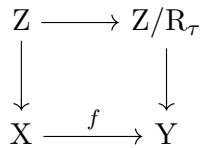
\includegraphics[keepaspectratio]{images/part003_fd3d7e4d.jpg}}

是笛卡尔方形。于是命题 6（IV, 第~391~页）的假设得到满足。因此，\(Z/R_{\tau}\) 是 Y 的覆叠。

命题 7. --- 设 X 和 Y 是拓扑空间，设 \(f: X \to Y\) 是连续且满射的映射。假设 Y 是可解圈的，且映射 f 是开映射并具有道路提升性质。那么，关于 f 在 X 的覆叠上的每个下降数据都是有效的，且商空间是 Y 的覆叠。

设 \((Z,p)\) 是 X 的覆叠，\(\tau\) 是关于 f 在 Z 上的下降数据。由于映射 f 满射且开，根据 IV, 第~389~页命题 5，下降数据 \(\tau\) 是有效的。令 \(T = Y/R_{\tau}\) 表示商 Y-空间；其投影 q 是平展的（同上），也是分离的（I, 第~27~页，命题 4）。

根据假设，映射 f 具有道路提升性质；映射 p 也有，因为 Z 是 X 的覆叠（III, 第~302~页，命题 3 的推论 2）。因此映射 \(p \circ f\) 也具有这一性质，从而映射 q 也有。于是（参见 IV, 第~341~页，注 2），T 是 Y 的覆叠。命题得证。

注。--- 设 X 和 Y 是拓扑空间，设 \(f: X \rightarrow Y\) 是映射。要使关于 f 在 X 的覆叠上的每个下降数据都有效且商空间是 Y 的覆叠，必要条件是 f 严格，并且 \(f(X)\) 是 X 的开闭子集。

事实上，将 X-空间 X 识别为 \(X \times_{Y} Y\)，并赋予它关于 f 的规范下降数据。商空间可识别为 \(f(\mathrm{X})\)，它带有由 f 定义的等价关系下从 X 的拓扑得到的商拓扑。若这是 Y 的覆叠，则空间 \(f(\mathrm{X})\) 可识别为 Y 的开闭子集，而映射 f 是严格的。

